\documentclass[a4paper,12pt]{report}
\usepackage[T1]{fontenc}
\usepackage[utf8]{inputenc}
\usepackage[italian]{babel}
\usepackage{graphicx, amsmath, amssymb, listings, eurosym}


\title{\textbf{{\huge {\huge CD \& DVD Shop Online}}} \\ Ingegneria del Software}
\author{
\includegraphics[scale=7.0]{Sfondo}
	\\ \\ \\
	Colognese Marco VR386474\\
	Rossini Mattia VR386327}
\date{}

\begin{document}
	
	\maketitle
	
	
	\tableofcontents
	
	
	
	\chapter*{Specifica}
	\addcontentsline{toc}{chapter}{Specifica}
	\small{Si vuole progettare un sistema informativo per gestire le informazioni relative alla gestione di un negozio virtuale di CD e DVD musicali (vende solo via web).\\
	Il negozio mette in vendita CD di diversi generi: jazz, rock, classica, latin, folk, world-music, e così via. Per ogni CD o DVD il sistema memorizza: un codice univoco, il titolo, i titoli di tutti i pezzi contenuti, eventuali fotografie della copertina, il prezzo, la data dalla quale è presente sul sito web del negozio, il musicista/band titolare, una descrizione, il genere del CD o DVD, i musicisti che vi suonano, con il dettaglio degli strumenti musicali usati. Per ogni musicista il sistema registra il nome d’arte, il genere principale, l’anno di nascita, se noto, gli strumenti che suona. Sul sito web del negozio è illustrato il catalogo dei prodotti in vendita. Cliccando sul nome del prodotto, appare una finestra con i dettagli del prodotto stesso.\\
	I clienti possono acquistare on-line selezionando gli oggetti da mettere in un “carrello della spesa” virtuale. Deve essere possibile visualizzare il contenuto del carrello, modificare il contenuto del carrello, togliendo alcuni articoli. Al termine dell’acquisto va gestito il pagamento, che può avvenire con diverse modalità.\\
	Il sistema supporta differenti ricerche: per genere, per titolare del CD o DVD, per musicista partecipante, per prezzo. Coerentemente, differenti modalità di visualizzazione, sono altresì supportate.\\
	Ogni vendita viene registrata indicando il cliente che ha acquistato, i prodotti acquistati, il prezzo complessivo, la data di acquisto, l’ora, l’indirizzo IP del PC da cui è stato effettuato l’acquisto, la modalità di pagamento (bonifico, carta di credito, Paypal) e la modalità di consegna (corriere, posta).\\
	Per ogni cliente il sistema registra: il suo codice fiscale, il nome utente (univoco) con cui si è registrato, la sua password, il nome, il cognome, la città di residenza, il numero di telefono ed eventualmente il numero di cellulare.\\
	Per i clienti autenticati, il sistema propone pagine specializzate che mostrano suggerimenti basati sul genere dei precedenti prodotti acquistati. Se il cliente ha fatto già 3 acquisti superiori ai 250 euro l’uno entro l’anno, il sistema gli propone sconti e consegna senza spese di spedizione.\\	
	Il personale autorizzato del negozio può inserire tutti i dati dei CD e DVD in vendita. Il personale
	inserisce anche il numero di pezzi a magazzino. Il sistema tiene aggiornato il numero dei pezzi a
	magazzino durante la vendita e avvisa il personale del negozio quando un articolo (CD o DVD) scende sotto i 2 pezzi in magazzino.}
	
	
	
	\chapter*{Analisi dei requisiti}
	\addcontentsline{toc}{chapter}{Analisi dei requisiti}
	Di seguito sono riportati i \textit{requisiti funzionali} del software realizzato.
	
	\begin{enumerate}
		\item Gli utenti che si interfacciano al sistema devono aver la possibilità di visualizzare il catalogo che mostra i prodotti (CD/DVD) salvati nel database. Cliccando su un prodotto, il sistema deve mostrare la scheda con i dettagli del CD/DVD.\\
		Il sistema deve inoltre permettere di effettuare ricerche che permettano di filtrare i prodotti del catalogo secondo alcuni criteri.
		
		\item Il sistema deve permettere a tutti gli utenti di registrarsi o autenticarsi tramite credenziali. Una volta autenticato l'utente acquisirà i permessi di cliente oppure di personale autorizzato.
		
		\item Il cliente può visualizzare un catalogo personale generato in base ai suoi precedenti acquisti. Il sistema riporterà anche degli sconti se il cliente ha già effettuato almeno 3 acquisti che superano i \euro$250$ entro l'anno.\\
		I clienti possono acquistare on-line selezionando gli oggetti da mettere in un “carrello della spesa” virtuale.\\
		Deve essere possibile visualizzare il contenuto del carrello, modificare il contenuto del carrello, togliendo alcuni articoli. Al termine dell’acquisto va gestito il pagamento, che può avvenire con diverse modalità.\\
		Ogni vendita viene registrata indicando il cliente che ha acquistato, i prodotti acquistati, il prezzo complessivo, la data di acquisto, l’ora, l’indirizzo IP del PC da cui è stato effettuato l’acquisto, la modalità di pagamento (bonifico, carta di credito, Paypal) e la modalità di consegna (corriere, posta).
		
		\item Il personale autorizzato ad ogni accesso riceverà una notifica nel caso in cui le scorte di 1 o più prodotti scendano sotto i 3 pezzi e potrà decidere di modificarle.\\
		Ha anche la possibilità di inserire un musicista nel database indicando il nome d’arte, il genere principale, l’anno di nascita e, se noto, gli strumenti che suona. Infine può inserire un prodotto nel database del sistema indicando un codice univoco, il titolo, i titoli di tutti i pezzi contenuti,
		eventuale fotografia della copertina, il prezzo, la data dalla quale è presente sul sito web del negozio, il musicista/band titolare, una descrizione, il genere del CD o DVD, i musicisti che vi suonano, con il dettaglio degli strumenti musicali usati.
	\end{enumerate}

	\section*{Interpretazione dei requisiti e scelte progettuali}
	\addcontentsline{toc}{section}{Interpretazione dei requisiti e scelte progettuali}
	Di seguito sono riportate le scelte progettuali effettuate dopo l'interpretazione dei requisiti del sistema:
	\begin{itemize}
		\item ogni utente che si interfaccia con il sito web può visualizzare il catalogo, effettuare ricerche e richiedere le schede con i dettagli dei prodotti anche se non si è autenticato;
		\item ogni utente che effettua la registrazione al sito viene anche automaticamente \textit{loggato} attraverso le sue credenziali;
		\item la ricerca è implementata attraverso l'applicazione di filtri al catalogo, e non come riordinamento dello stesso, variandone dunque la modalità di visualizzazione;
		\item il catalogo personale di un cliente viene generato facendo riferimento alla storia dei suoi acquisti e mettendo in primo piano i CD/DVD del genere più acquistato;
		\item gli sconti per i clienti che hanno effettuato almeno 3 acquisti da \euro{}$250$ entro l'anno vengono riportati direttamente sul catalogo;
		\item il personale autorizzato può inserire anche dei musicisti nel database del sistema oltre ai prodotti e variare le scorte.
	\end{itemize}
	
	
	
	\chapter*{Use Case}
	\addcontentsline{toc}{chapter}{Use Case}
	\section*{UC1: Catalogo}
	\addcontentsline{toc}{section}{UC1: Catalogo}
	\noindent
	\textbf{Caso d'uso:} Catalogo\\
	\textbf{Id:} UC1\\
	\textbf{Attori:} Utente\\
	\textbf{Precondizioni:} L'utente si collega alla pagina web del negozio\\
	\textbf{Sequenza di eventi:}
	\begin{enumerate} 
		\item Il caso d'uso inizia quando l'utente si collega alla pagina web del negozio
		\item Il sistema visualizza il catalogo
		\item Se l'utente clicca sul prodotto:
		\begin{enumerate} 
			\item il sistema visualizza la rispettiva scheda prodotto
		\end{enumerate}
		\item Se l'utente esegue una ricerca attraverso dei filtri:
		\begin{enumerate}
			\item il sistema filtra il catalogo in base alle richieste dell'utente
		\end{enumerate}
		\end{enumerate}
	\textbf{Postcondizioni:} l'utente visualizzerà 0 o più prodotti\\
	\textbf{Sequenza alternativa:}
	\begin{enumerate}
		\item in qualunque momento l'utente può abbandonare la pagina di ricerca.
	\end{enumerate}

	\begin{figure}[h]
		\centering
		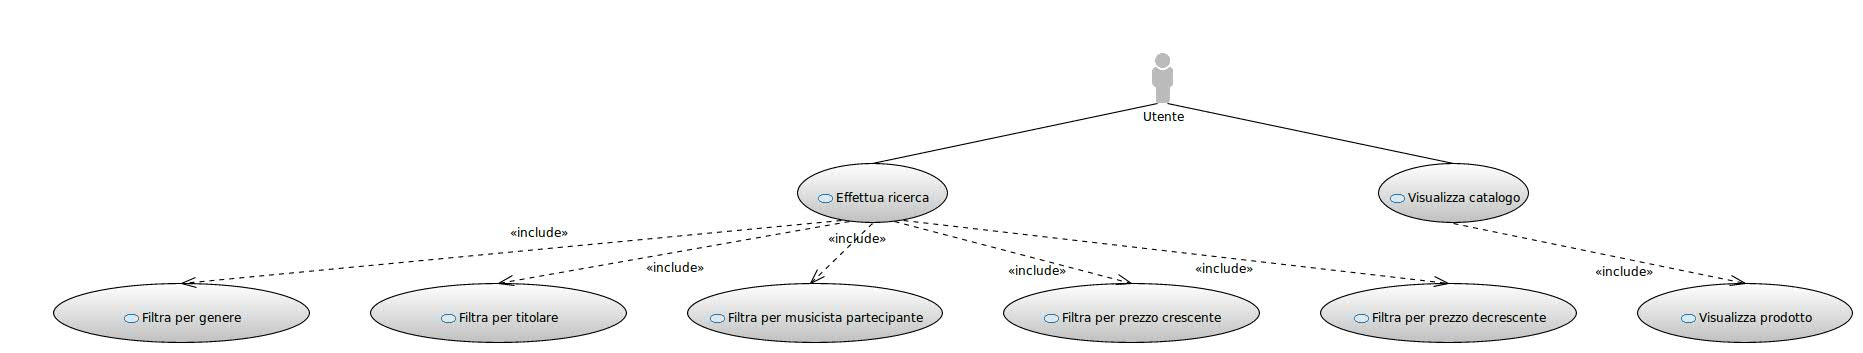
\includegraphics[width=\textwidth, height=4.104cm]{Catalogo}
	\end{figure}

	\newpage
	\section*{UC2: Cliente}
	\addcontentsline{toc}{section}{UC2: Cliente}
	\noindent
	\textbf{Caso d'uso:} Cliente\\
	\textbf{Id:} UC2\\
	\textbf{Attori:} Utente, Cliente, Personale autorizzato\\
	\textbf{Precondizioni:} L'utente si collega alla pagina web del negozio\\
	\textbf{Sequenza di eventi:}
	\begin{enumerate} 
		\item Il caso d'uso inizia quando l'utente decide di registrarsi o autenticarsi
		\item Se l'utente decide di registrarsi e diventare cliente:
		\begin{enumerate}
			\item dovrà fornire al sistema tutti i dati necessari per la registrazione
		\end{enumerate}
		\item Se l'utente decide di autenticarsi e diventare cliente:
		\begin{enumerate}
			\item dovrà fornire al sistema i dati necessari per l'autenticazione
		\end{enumerate}
		\item Se l'utente si è autenticato:
		\begin{enumerate}
			\item il sistema gli propone un catalogo personalizzato
		\end{enumerate}
		\item Se l'utente ha effettuato almeno 3 spese superiori ai \euro$250.00$ entro l'anno:
		\begin{enumerate}
			\item il sistema gli propone degli sconti personalizzati
		\end{enumerate}
	\end{enumerate}
	\textbf{Postcondizioni:} il cliente può effettuare acquisti sul sito.
	
	\begin{figure}[h]
		\centering
		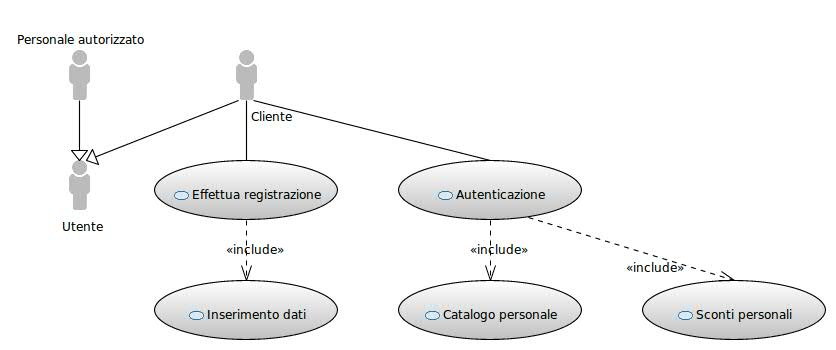
\includegraphics[width=\textwidth]{Cliente}
	\end{figure}
	
	\newpage
	\section*{UC3: Carrello}
	\addcontentsline{toc}{section}{UC3: Carrello}
	\noindent
	\textbf{Caso d'uso:} Carrello\\
	\textbf{Id:} UC3\\
	\textbf{Attori:} Cliente\\
	\textbf{Precondizioni:} L'utente, dopo aver effettuato l'accesso tramite le sue credenziali, ha trovato qualcosa a cui è interessato\\
	\textbf{Sequenza di eventi:}
	\begin{enumerate} 
		\item Il caso d'uso inizia quando il cliente aggiunge al carrello i prodotti
		\item In caso di errore, il cliente modifica il carrello
		\item Sceglie la modalità di spedizione
		\item Effettua il pagamento, scegliendo la modalità
	\end{enumerate}
	\textbf{Postcondizioni:} l'ordine è stato creato.
	
	\begin{figure}[h]
		\centering
		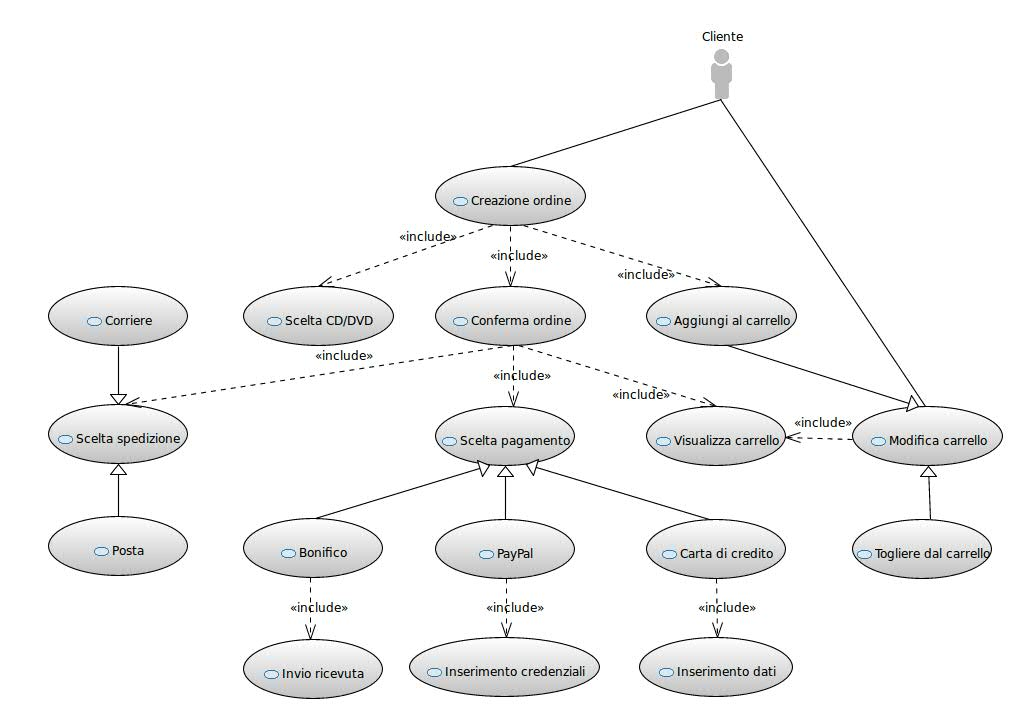
\includegraphics[width=\textwidth]{Carrello}
	\end{figure}
	
	\newpage
	\section*{UC4: Personale autorizzato}
	\addcontentsline{toc}{section}{UC4: Personale autorizzato}
	\noindent
	\textbf{Caso d'uso:} Personale autorizzato\\
	\textbf{Id:} UC4\\
	\textbf{Attori:} Personale autorizzato\\
	\textbf{Precondizioni:} L'utente si autentica come personale autorizzato attraverso le sue credenziali di accesso\\
	\textbf{Sequenza di eventi:}
	\begin{enumerate} 
		\item Il caso d'uso inizia quando l'utente effettua con successo il login come personale autorizzato
		\item Il personale autorizzato può ricevere una notifica se le scorte in magazzino di qualche prodotto stanno terminando
		\item Se il personale autorizzato gestisce il magazzino:
		\begin{enumerate}
			\item aggiorna le scorte dei prodotti nel magazzino
		\end{enumerate}
		\item Se il personale autorizzato registra un musicista nel database del negozio:
		\begin{enumerate}
			\item deve inserire le informazioni del musicista
			\item conferma l'inserimento
		\end{enumerate}
		\item Se il personale autorizzato registra un prodotto (CD/DVD) nel database del negozio:
		\begin{enumerate}
			\item deve inserire le informazioni del prodotto
			\item può inserire la copertina
			\item conferma l'inserimento
		\end{enumerate}
	\end{enumerate}
	\textbf{Postcondizioni:} il magazzino viene aggiornato.
	
	\begin{figure}[h]
		\centering
		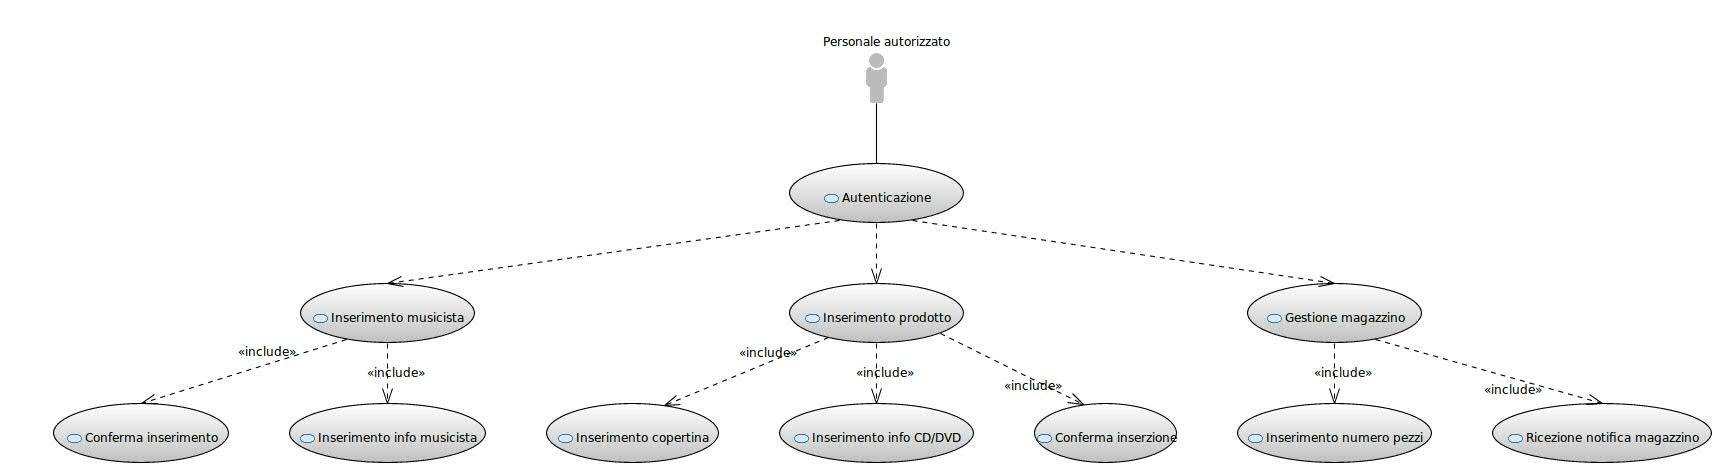
\includegraphics[width=\textwidth, height=5cm]{PersonaleAutorizzato}
	\end{figure}



	\chapter*{Sequence Diagram}
	\addcontentsline{toc}{chapter}{Sequence Diagram}
	\section*{Catalogo}
	\addcontentsline{toc}{section}{Catalogo}
	\begin{figure}[h]
		\centering
		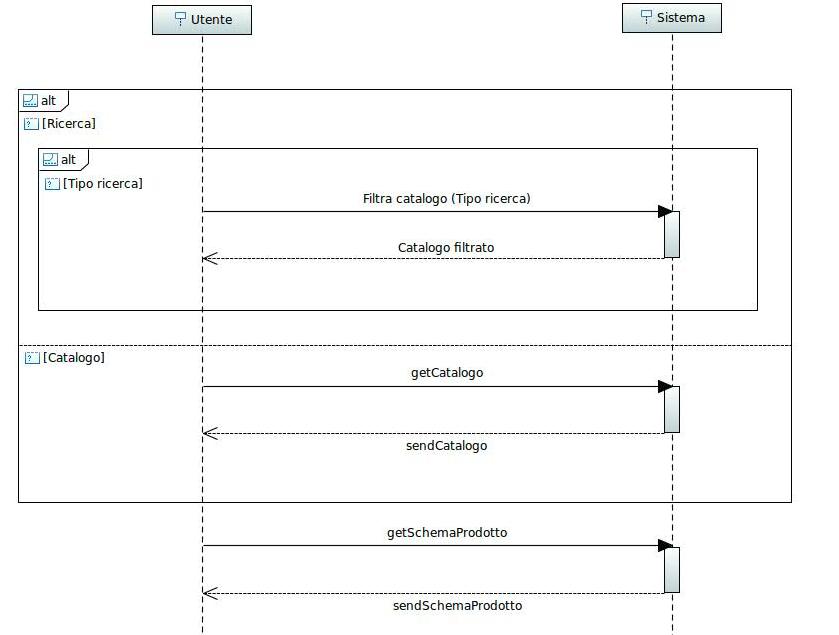
\includegraphics[width=\textwidth, height=13cm]{Sequence_Utente}
	\end{figure}
	
	\newpage
	\section*{Cliente}
	\addcontentsline{toc}{section}{Cliente}
	\begin{figure}[h]
		\centering
		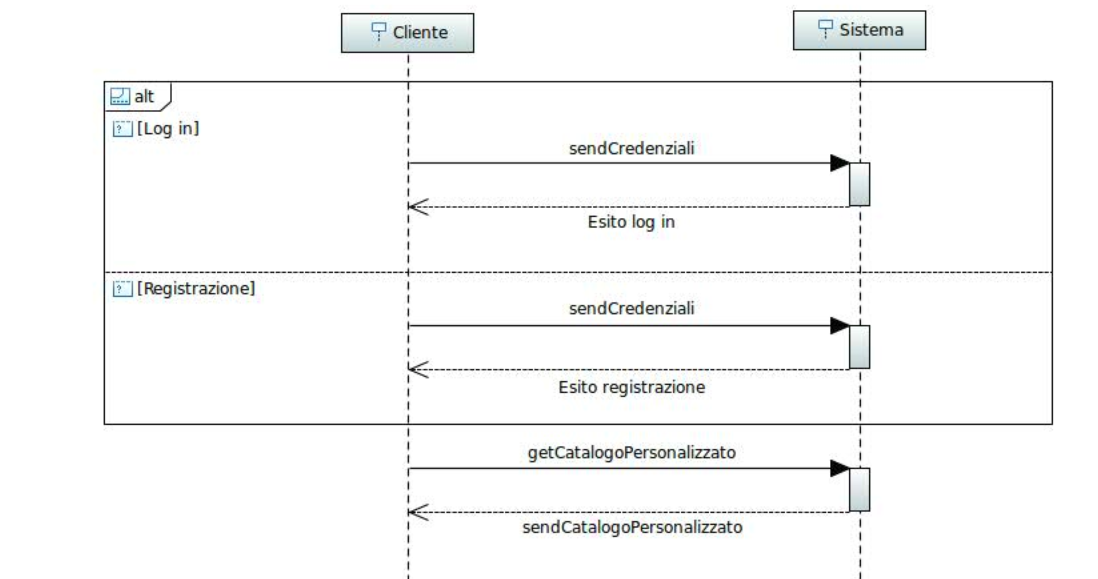
\includegraphics[width=\textwidth, height=12cm]{Sequence_Cliente}
	\end{figure}
	
	\newpage
	\section*{Carrello}
	\addcontentsline{toc}{section}{Carrello}
	\begin{figure}[h]
		\centering
		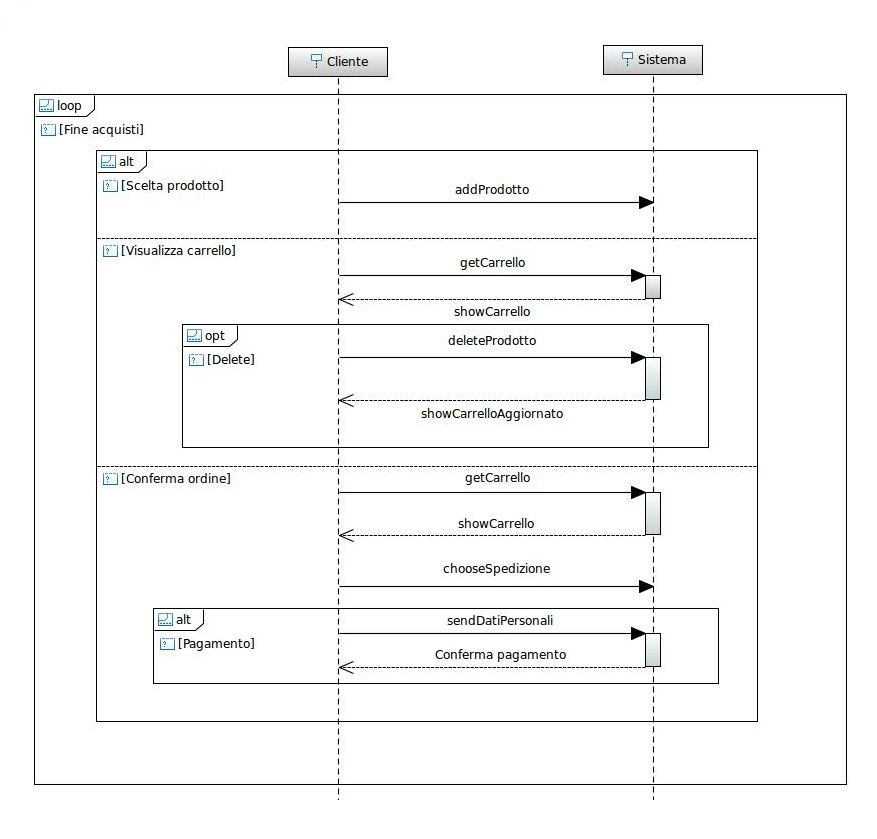
\includegraphics[width=\textwidth, height=16cm]{Sequence_Ordine}
	\end{figure}
	
	\newpage
	\section*{Personale autorizzato}
	\addcontentsline{toc}{section}{Personale autorizzato}
	\begin{figure}[h]
		\centering
		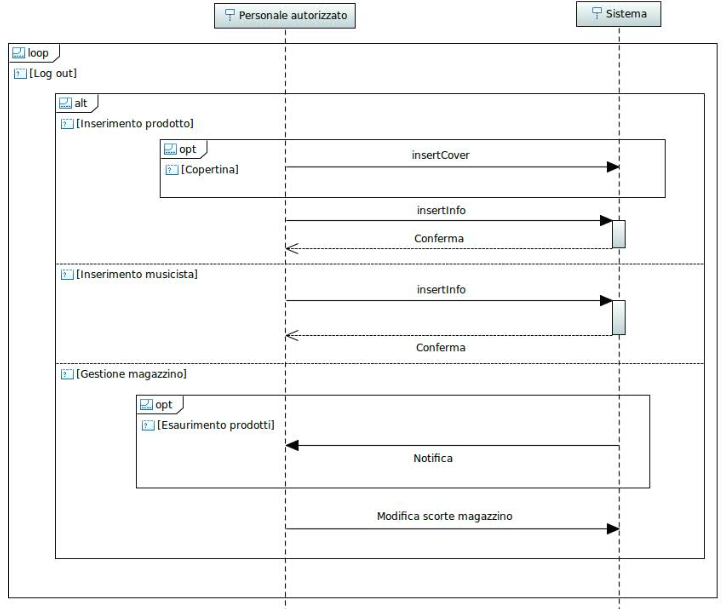
\includegraphics[width=\textwidth, height=15cm]{Sequence_Gestore}
	\end{figure}



	\chapter*{Activity Diagram}
	\addcontentsline{toc}{chapter}{Activity Diagram}
	\section*{Catalogo}
	\addcontentsline{toc}{section}{Catalogo}
	\begin{figure}[h]
		\centering
		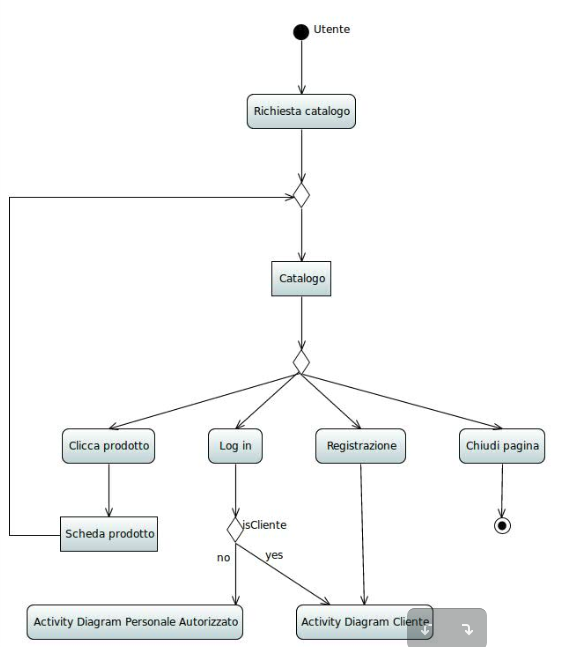
\includegraphics[scale=0.6, height=13cm]{Activity_Catalogo}
	\end{figure}
	
	\newpage
	\section*{Cliente}
	\addcontentsline{toc}{section}{Cliente}
	\begin{figure}[h]
		\centering
		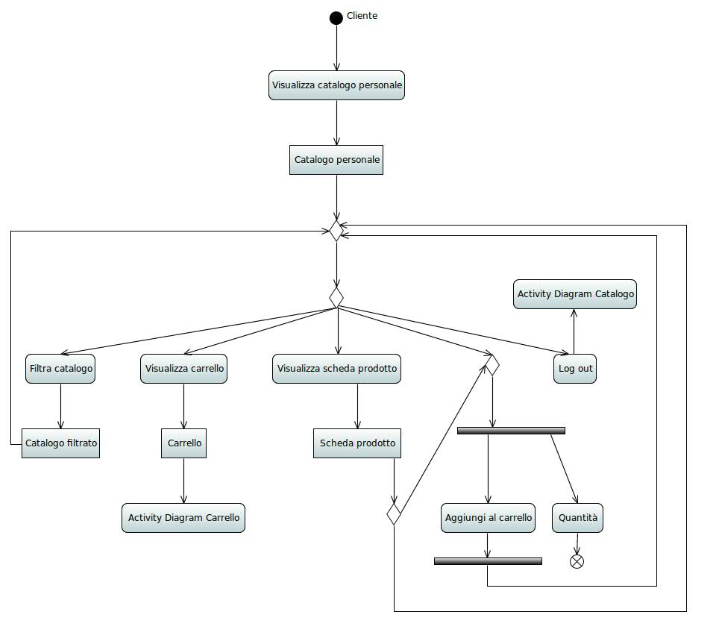
\includegraphics[width=\textwidth, height=16cm]{Activity_Cliente}
	\end{figure}
	
	\newpage
	\section*{Carrello}
	\addcontentsline{toc}{section}{Carrello}
	\begin{figure}[h]
		\centering
		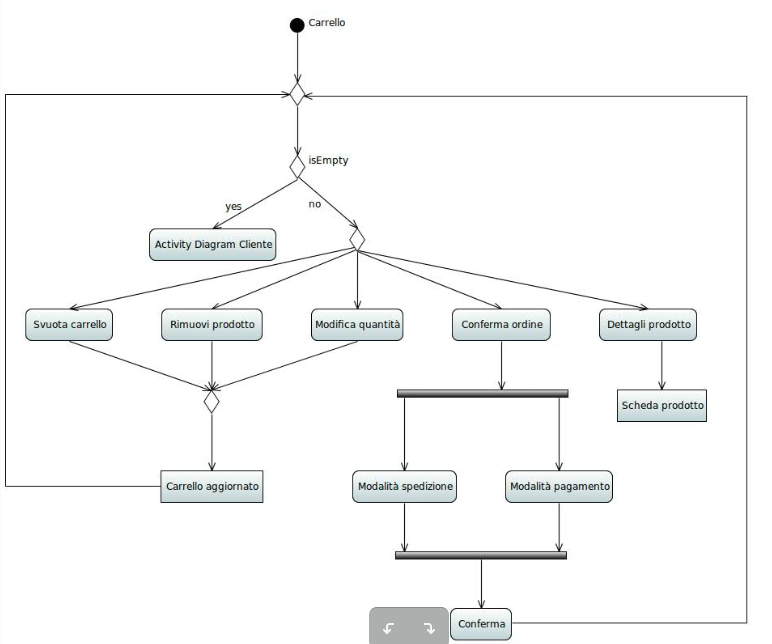
\includegraphics[width=\textwidth, height=16cm]{Activity_Carrello}
	\end{figure}
	
	\newpage
	\section*{Personale autorizzato}
	\addcontentsline{toc}{section}{Personale autorizzato}
	\begin{figure}[h]
		\centering
		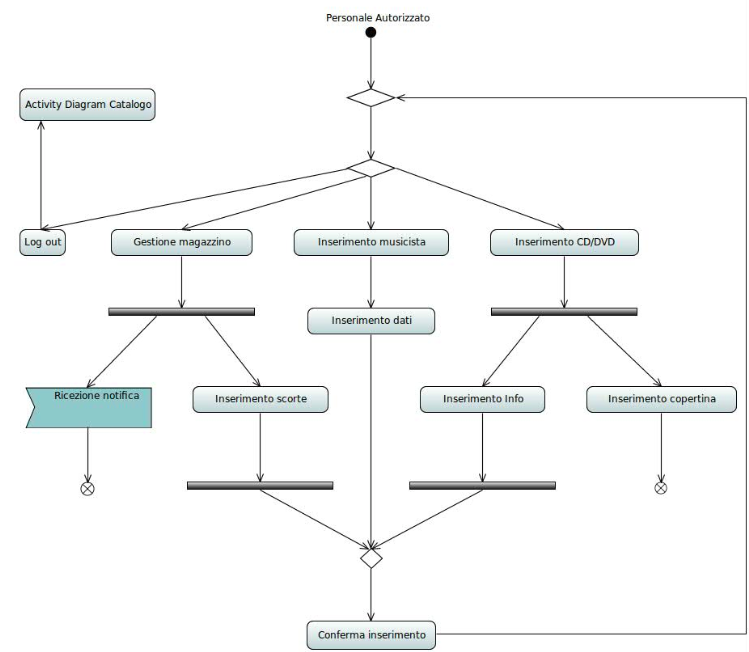
\includegraphics[width=\textwidth, height=16cm]{Activity_PersonaleAutorizzato}
	\end{figure}



	\chapter*{Class Diagram}
	\addcontentsline{toc}{chapter}{Class Diagram}
	\begin{figure}[h]
		\centering
		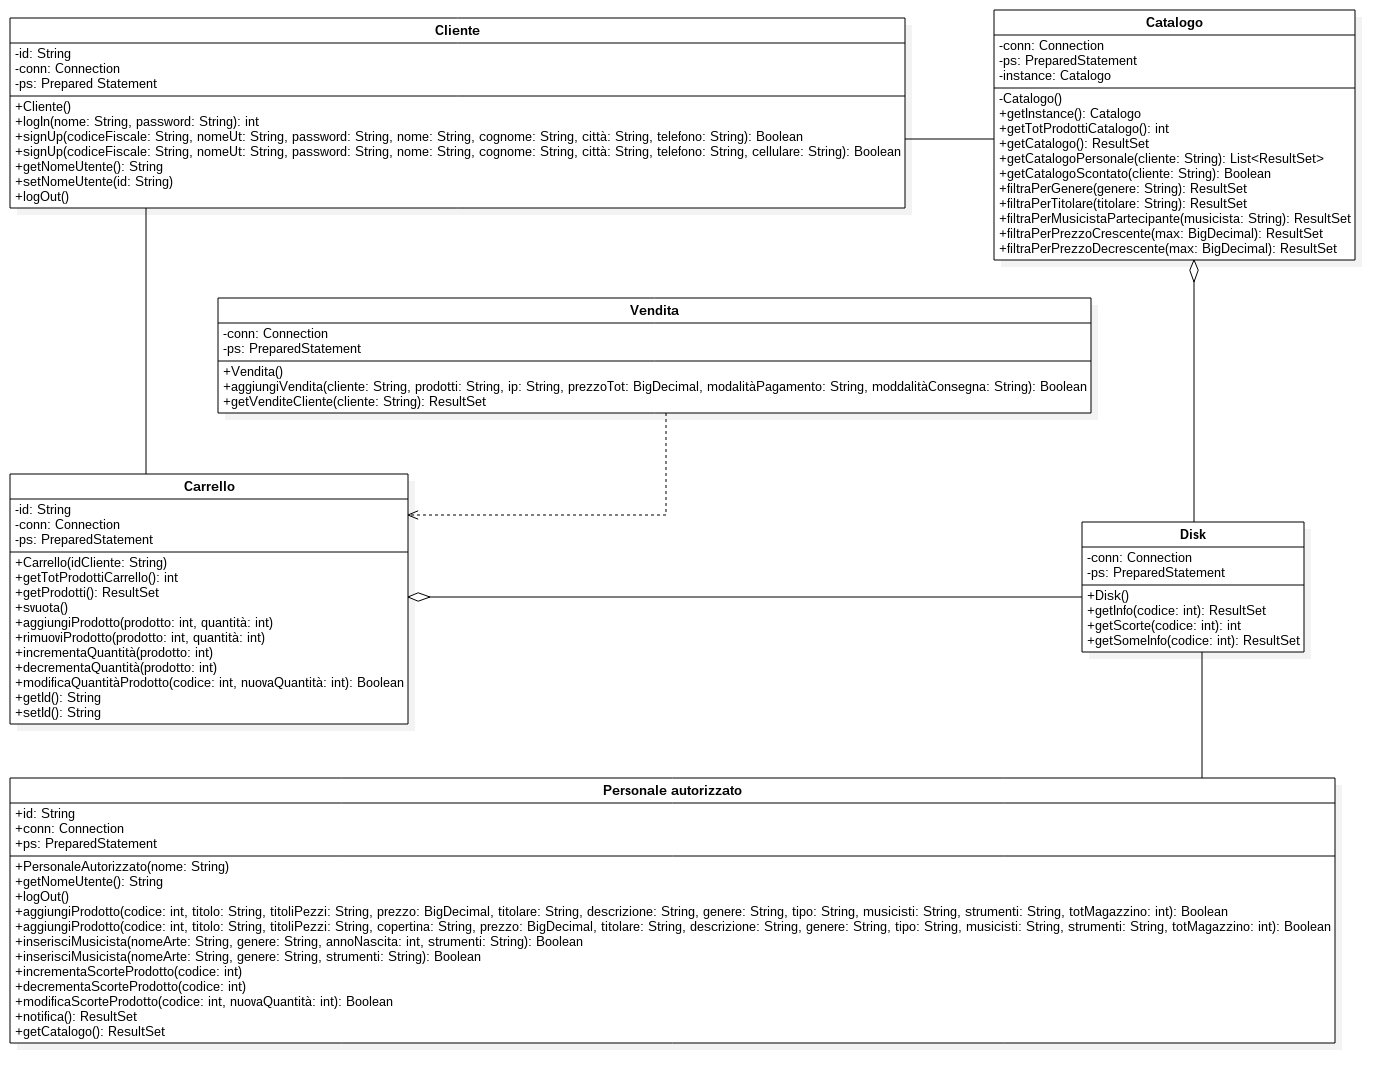
\includegraphics[width=17cm, height=15cm]{Class}
	\end{figure}
	
	
	
	\chapter*{Design Pattern}
	\addcontentsline{toc}{chapter}{Design Pattern}
	In questo progetto sono stati implementati due design pattern: \textit{Singleton} per la classe Catalogo, \textit{Proxy} per il catalogo visualizzato dal Personale Autorizzato.\\ \\
	\textit{Proxy} è invece utilizzato per caricare il catalogo del personale autorizzato e lo tiene salvato fino a quando non viene modificato. In questo modo si evita di caricarlo inutilmente dal database anche quando non è stato modificato.
	\\
	\newline
	\textit{Singleton} è usato per assicurare che una classe abbia una sola istanza ed un unico punto di accesso globale.\\
	In molte situazioni c’è la necessità di garantire l’esistenza di un unico oggetto di una classe: nel nostro caso la classe Catalogo deve avere un'unica istanza.\\
	Le classi Singleton vengono progettate con i costruttori privati per evitare la possibilità di istanziare un numero arbitrario di oggetti della stessa.\\
	Esiste un metodo statico con la responsabilità di assicurare che nessuna altra istanza venga creata oltre la prima, restituendo contemporaneamente un riferimento all’unica esistente.\\
	La classe mantiene all’interno il riferimento all’unica istanza Singleton della classe (quella creata alla prima esecuzione del metodo statico).\\
	La classe contiene poi tutti i metodi, le proprietà e gli attributi tipici dell’astrazione per cui è
	stata concepita.
	\newline
	\newline
	\newline
	\textbf{Singleton implementato sulla classe \textit{Catalogo:}}	
	\begin{figure}[h]
		\centering
		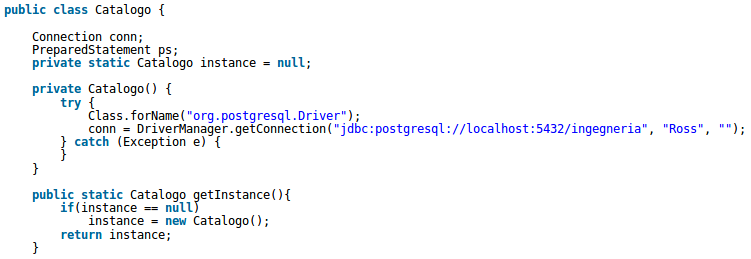
\includegraphics[width=\textwidth, height=4cm]{Singleton}
	\end{figure}
	
	
	
	\chapter*{Pattern architetturale}
	\addcontentsline{toc}{chapter}{Pattern architetturale}
	In questo progetto è presente un pattern architetturale utile per separare la logica di presentazione dei dati (interfaccia utente) dalla logica di business: il \textit{Model-View-Controller (MVC)}.\\
	Il pattern, implementato sul lato server è basato sulla separazione dei compiti fra i componenti software che svolgono i tre ruoli principali:
	\begin{itemize}
	\item il \textit{model} è il componente centrale del MVC e fornisce i metodi per accedere ai dati utili all'applicazione, cioè il database; cattura il comportamento dell'applicazione indipendentemente dall'interfaccia utente.
	\item la \textit{view} può essere una qualsiasi rappresentazione in output di informazioni (sono possibili viste multiple per le stesse informazioni); visualizza i dati contenuti nel model e si occupa dell'interazione con l'utente.
	\item il \textit{controller} riceve i comandi dell'utente (attraverso la \textit{view}) e li converte in comandi per il modello.
	\end{itemize}
	\begin{figure}[h]
		\centering
		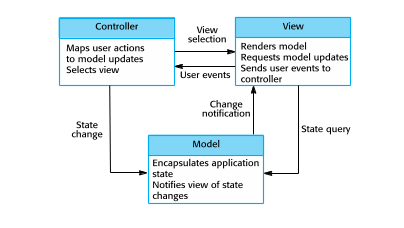
\includegraphics[scale=0.94]{MVC}
	\end{figure}



		
	
	
	\chapter*{Unit \& System Tests}
	\addcontentsline{toc}{chapter}{Unit \& System Tests}
	I test dell'interfaccia grafica sono stati eseguiti sin dall'inizio del progetto e sono continuati durante tutto il suo sviluppo, cercando di provare tutte le possibili situazioni in cui un utente può trovarsi.
	\\
	Allo stesso modo sono state testate tutte le classi che si interfacciano con il database per evitare ogni possibile errore di aggiornamento dei record del database ed eventuali violazioni sui domini.
	\newline
	\newline
	I test sul prodotto finale sono stati eseguiti per cercare eventuali bug e funzionamenti indesiderati che non sono stati individuati dai test sulle varie unità del progetto.
	\newline
	\newline
	Ogni classe e metodo è stato testato direttamente durante l'implementazione senza il supporto di software per l'automatizzazione dei test (come JUnit).
	\\
	Questa scelta deriva dal fatto che il progetto non è di grandi dimensioni e l'implementazione di classi per i test sui metodi avrebbe comportato un maggior dispendio di tempo.

	
	
\end{document}